\documentclass[conference]{IEEEtran}

% -----------------------------------------------------------------------
% Packages
% -----------------------------------------------------------------------
\usepackage[T1]{fontenc}
\usepackage[utf8]{inputenc}
\usepackage{amsmath,amssymb}
\usepackage{graphicx}
\usepackage{booktabs}
\usepackage{siunitx}
\usepackage{array}
\usepackage{xcolor}
\usepackage{algorithm}
\usepackage{algpseudocode}
\usepackage{tikz}
\usepackage{pgfplots}
\pgfplotsset{compat=1.18}
\usepackage{cite}
\usepackage{url}
\usepackage{microtype}
\usepackage{balance}

\usetikzlibrary{shapes.geometric, arrows.meta, positioning, fit,
                backgrounds, decorations.pathreplacing, calc}

\tikzset{
  block/.style  = {rectangle, rounded corners=3pt, draw=gray!60,
                   fill=blue!6, text width=2.8cm, align=center,
                   minimum height=0.65cm, font=\scriptsize},
  sblock/.style = {rectangle, rounded corners=2pt, draw=gray!50,
                   fill=green!8, text width=2.4cm, align=center,
                   minimum height=0.6cm, font=\scriptsize},
  arrow/.style  = {->, >=Stealth, thick},
  dline/.style  = {dashed, gray!55},
}

% -----------------------------------------------------------------------
\begin{document}

\title{TRAW: Traffic-Aware Multi-Pass RAW Scheduling\\
with Periodic Sleep for Dense IEEE~802.11ah IoT Networks}

\author{
  \IEEEauthorblockN{Alakesh Kalita,~\IEEEmembership{Senior Member,~IEEE,}
    and Nurzaman Ahmed,~\IEEEmembership{Member,~IEEE}}
  \IEEEauthorblockA{Department of Mathematics and Computing,
    Indian Institute of Technology (ISM) Dhanbad, India\\
    \{alakesh.kalita1025, nurzaman713\}@gmail.com}
}

\maketitle

% -----------------------------------------------------------------------
\begin{abstract}
Dense IEEE~802.11ah (Wi-Fi HaLow) IoT deployments face a fundamental
tension between high-traffic groups that require multiple channel-access
opportunities per beacon interval and idle groups that waste beacon
budget on empty transmission windows.
This paper proposes TRAW (\emph{Traffic-aware RAW}), a standard-compliant
access-point scheduler that addresses this tension through three
coordinated mechanisms built on CUSUM-boosted EWMA per-station demand
prediction: \emph{(A)} demand-proportional slot allocation that
distributes the beacon budget among groups according to predicted load;
\emph{(B)} multi-pass scheduling that issues a second RAW window within
the same beacon interval for groups whose per-AID demand exceeds a
configurable threshold, doubling their channel-access opportunities; and
\emph{(C)} Periodic~RAW (PRAW, IEEE~802.11ah \S9.4.2.200) skip that
suspends idle groups to every $P$-th beacon interval, freeing recovered
budget for congested peers.
A beacon-budget group-count bound ensures all windows fit within the
beacon interval regardless of load conditions, and a budget-safe split
feasibility check prevents structural group changes from triggering
catastrophic slot-duration inflation.
Simulations over $N\!\in\!\{100,\ldots,1000\}$ stations show TRAW
achieves PDR gains of 12\,\% ($N\!=\!400$), 43\,\% ($N\!=\!600$),
and 113\,\% ($N\!=\!800$) over the prior TASM-RAW policy, while
maintaining comparable performance at light loads ($N\!\leq\!200$).
At $N\!=\!800$ TRAW achieves PDR\,=\,0.384, outperforming all five
baseline policies.
\end{abstract}

\begin{IEEEkeywords}
IEEE 802.11ah, Wi-Fi HaLow, RAW, restricted access window, PRAW,
multi-pass scheduling, demand-proportional allocation, CUSUM-EWMA,
IoT, dense networks, beacon scheduling.
\end{IEEEkeywords}

% -----------------------------------------------------------------------
\section{Introduction}
\label{sec:intro}

The IEEE~802.11ah standard (Wi-Fi HaLow)~\cite{std80211ah} is designed
for large-scale IoT deployments where hundreds of low-power sensors
share a sub-1\,GHz channel.
Its Restricted Access Window (RAW) mechanism partitions the post-beacon
contention period into non-overlapping group windows, each serving a
disjoint AID range, reducing the number of simultaneous contenders from
$N$ to roughly $N/G$ and suppressing collision-driven throughput
collapse.

\textbf{Limitations of uniform-window RAW.}
Existing RAW policies---static, adaptive single-group, and dynamic
split-merge (TASM-RAW~\cite{kalita2025b})---all share one key assumption:
every active group receives a single transmission window per beacon
interval (BI), and all windows have the same sub-slot count $S$.
This is inefficient in two orthogonal ways.
First, \emph{high-demand groups} (e.g., a cluster of sensors near a
deadline) contend against each other in one window when a second window
in the same BI would dramatically improve delivery probability.
Second, \emph{idle groups} (sensors in sleep-heavy duty cycles)
consume a full window slot every BI even though they carry essentially
zero traffic, wasting precious beacon budget.

\textbf{The PRAW opportunity.}
The 802.11ah standard~\cite{std80211ah} already provides a mechanism to
address idle groups: the Periodic~RAW (PRAW) option in the RAW
Parameter Set element (\S9.4.2.200) allows a group to be active only
once every $P$ BIs, with the remaining $P-1$ BIs skipped entirely.
No prior dynamic policy exploits PRAW for idle-group suppression
in a fully adaptive per-beacon scheduler.

\textbf{Contributions.}
This paper proposes TRAW, a traffic-aware RAW policy that jointly adapts
group boundaries, slot durations, sub-slot counts, multi-pass windows,
and PRAW phases at every beacon epoch.
The main contributions are:
\begin{itemize}
  \item A \emph{demand-proportional slot allocation} (mechanism A) that
        redistributes beacon budget from low-demand groups to high-demand
        ones using a floor-protected share formula, ensuring no group
        falls below a configurable minimum while busy groups receive
        proportionally more airtime.
  \item A \emph{multi-pass second-window scheduler} (mechanism B) that
        pre-reserves a fraction of the beacon budget and issues a
        second RawConfig entry for groups whose per-AID demand exceeds
        a threshold, giving them twice as many channel-access
        opportunities within a single BI without requiring any
        standard extension.
  \item A \emph{PRAW-based idle-group suppression} (mechanism C) that
        suspends groups with near-zero EWMA demand after a confirmation
        window, activating them only once every $P$ BIs; a warmup guard
        prevents premature entry during EWMA transients, and an
        immediate wakeup triggers when demand recovers.
  \item A \emph{budget-safe split feasibility criterion} that uses
        $D_\mathrm{min}$ (T* at $n\!=\!1$) rather than the
        backlog-inflated T* when checking whether a proposed split fits
        within the beacon budget, preventing split rejection under
        congestion and enabling healthy group count adaptation.
  \item A \emph{target-slots group count initialisation} that caps the
        initial number of groups at $\lfloor\eta T_B / (S_\mathrm{tgt}
        \times D_\mathrm{min})\rfloor$, matching the budget-allocation
        logic of TASM-RAW and preventing over-fragmentation at startup.
\end{itemize}

Simulation results show TRAW outperforms TASM-RAW (the strongest prior
policy) at every $N\!\geq\!400$ and significantly exceeds all five
baselines at $N\!\geq\!600$.

Section~\ref{sec:related} surveys related work.
Section~\ref{sec:model} defines the system model.
Section~\ref{sec:design} presents TRAW in detail.
Section~\ref{sec:eval} evaluates performance.
Section~\ref{sec:conc} concludes.

% -----------------------------------------------------------------------
\section{Related Work}
\label{sec:related}

\textbf{Static RAW.}
Tian et al.~\cite{tian2016} derive closed-form optimal group count and
slot duration for static saturated traffic; Raeesi et al.~\cite{raeesi2014}
show static RAW outperforms DCF beyond $N\!=\!50$ but degrades sharply
with parameter mismatch.
Both works fix $G$ and $D$ at deployment.

\textbf{Adaptive slot sizing.}
Bhandari and Moh~\cite{bhandari2018} adjust a single group's slot via
collision feedback.
Kalita and Ahmed~\cite{kalita2025} introduce a CUSUM-EWMA estimator for
per-STA demand that adapts slot duration without overhead; TRAW inherits
this estimator.
Taramit et al.~\cite{taramit2023} propose LACA, a renewal-process slot
model for a single fixed group; TRAW applies the same LACA formula
across dynamically-sized groups.

\textbf{Dynamic grouping.}
Kim and Moh~\cite{kim2017} use pre-provisioned cluster assignments;
Chang et al.~\cite{chang2019} collect per-STA reports via management
frames, incurring overhead incompatible with low-power nodes.
Kalita and Ahmed~\cite{kalita2025b} (TASM-RAW) combine CUSUM-EWMA
prediction with load-median split/merge to adapt both $G$ and $\{D_g\}$
per beacon; TRAW extends this base with multi-pass windows and PRAW.

\textbf{PRAW usage.}
The PRAW element (\S9.4.2.200)~\cite{std80211ah} is specified for
static provisioning of infrequent sensor groups.
We are not aware of any prior work that dynamically assigns PRAW
periodicity to groups based on live per-beacon demand estimates.

% -----------------------------------------------------------------------
\section{System Model}
\label{sec:model}

We consider a single-cell star BSS with one AP and $N$ uplink STAs.
All nodes use MCS0 (BPSK~$\frac{1}{2}$, 150\,kb/s) on a 915\,MHz
channel.
The AP broadcasts a DTIM beacon every $T_B\!=\!500$\,ms.
Each beacon embeds an RPS element that partitions AIDs
$\{1,\ldots,N\}$ into $G(t)$ non-overlapping contiguous groups
$\mathcal{G}(t)=\{[s_1,e_1],\ldots,[s_G,e_G]\}$, assigning each
group $g$ a sub-slot count $S_g(t)$ and slot duration $D_g(t)$.
STAs contend only during their assigned window; outside it they sleep.

At each beacon epoch $t$ the AP reads the MAC TX-queue depth
$q_i(t)$ of each associated STA $i$.
No additional signalling or explicit STA feedback is required.

\textbf{Design objective.}
Choose $G(t)$, $\{S_g(t)\}$, $\{D_g(t)\}$, and per-group PRAW
phases to maximise aggregate PDR subject to the feasibility constraint:
\begin{equation}
  \sum_{g=1}^{G(t)} S_g(t)\cdot D_g(t) \;\leq\; \eta\,T_B,
  \label{eq:feasibility}
\end{equation}
where $\eta\!=\!0.9$ reserves 10\,\% for beacon overhead and initial
backoff.

\textbf{PRAW mechanism.}
A group in PRAW mode is active on beacon $t$ if and only if
$(t \bmod P)\!=\!0$.
In the remaining $P-1$ BIs the group emits no RawConfig entry and
its STAs remain in deep sleep.
The freed budget $S_g\cdot D_g$ is available for other groups or
for multi-pass extra windows.

% -----------------------------------------------------------------------
\section{Proposed TRAW Scheme}
\label{sec:design}

Fig.~\ref{fig:arch} shows the per-beacon control flow of TRAW.
The AP executes seven steps at each beacon epoch, described in the
following subsections.

\begin{figure}[!t]
\centering
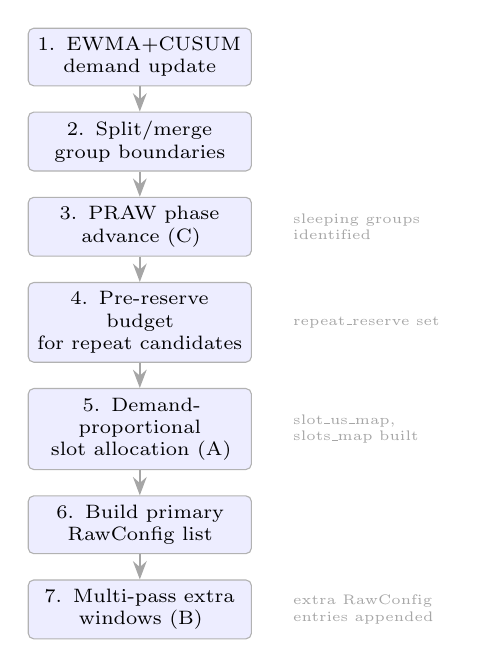
\begin{tikzpicture}[
  font=\scriptsize,
  node distance=0.32cm,
  box/.style={rectangle, rounded corners=2pt, draw=gray!60,
              fill=blue!7, text width=2.6cm, align=center,
              minimum height=0.55cm},
  arr/.style={->, >=Stealth, thick, gray!70},
]
  \node[box] (s1) {1. EWMA+CUSUM\\demand update};
  \node[box, below=of s1] (s2) {2. Split/merge\\group boundaries};
  \node[box, below=of s2] (s3) {3. PRAW phase\\advance (C)};
  \node[box, below=of s3] (s4) {4. Pre-reserve budget\\for repeat candidates};
  \node[box, below=of s4] (s5) {5. Demand-proportional\\slot allocation (A)};
  \node[box, below=of s5] (s6) {6. Build primary\\RawConfig list};
  \node[box, below=of s6] (s7) {7. Multi-pass extra\\windows (B)};

  \draw[arr] (s1)--(s2);
  \draw[arr] (s2)--(s3);
  \draw[arr] (s3)--(s4);
  \draw[arr] (s4)--(s5);
  \draw[arr] (s5)--(s6);
  \draw[arr] (s6)--(s7);

  \node[right=0.4cm of s3, font=\tiny, text=gray!70, align=left]
    {sleeping groups\\identified};
  \node[right=0.4cm of s4, font=\tiny, text=gray!70, align=left]
    {repeat\_reserve set};
  \node[right=0.4cm of s5, font=\tiny, text=gray!70, align=left]
    {slot\_us\_map,\\slots\_map built};
  \node[right=0.4cm of s7, font=\tiny, text=gray!70, align=left]
    {extra RawConfig\\entries appended};
\end{tikzpicture}
\caption{TRAW per-beacon control flow. Steps 1--2 are shared with
TASM-RAW~\protect\cite{kalita2025b}; steps 3--7 are new.}
\label{fig:arch}
\end{figure}

% ---------
\subsection{Traffic Demand Estimation}
\label{sec:demand}

Let $q_i(t)$ denote the MAC TX-queue depth of STA~$i$ at epoch $t$.
An EWMA smoother tracks the trend:
\begin{equation}
  \hat{q}_i(t) = \alpha\,q_i(t) + (1-\alpha)\,\hat{q}_i(t-1),
  \quad \alpha=0.3,
  \label{eq:ewma}
\end{equation}
and a one-sided CUSUM detects sustained upward deviations:
\begin{align}
  e_i(t)   &= q_i(t) - \hat{q}_i(t-1), \label{eq:err}\\
  C_i(t)   &= \max\!\bigl(0,\;C_i(t-1)+e_i(t)-k\bigr),\quad k=0.15.
  \label{eq:cusum}
\end{align}
The burst-boosted demand estimate is:
\begin{equation}
  d_i(t) = \max\!\bigl(0,\;\hat{q}_i(t)+\max(0,\,C_i(t)-h)\bigr),
  \quad h=0.8.
  \label{eq:demand}
\end{equation}
The CUSUM boost activates only after the queue has been consistently
elevated, providing robustness to isolated spikes.
The per-group aggregate load and normalised per-AID demand are:
\begin{equation}
  D_g(t) = \sum_{i=s_g}^{e_g} d_i(t), \quad
  \lambda_g(t) = \frac{D_g(t)}{e_g - s_g + 1}.
  \label{eq:group_load}
\end{equation}

% ---------
\subsection{Group Initialisation and Split/Merge}
\label{sec:split_merge}

\textbf{Initial group count.}
At startup, the number of groups is bounded by the target-slots
criterion:
\begin{equation}
  G_\mathrm{max}^\mathrm{init} = \min\!\left(
    \left\lfloor\frac{\eta\,T_B}{S_\mathrm{tgt}\cdot D_\mathrm{min}}\right\rfloor,\;
    \left\lfloor\frac{N}{n_\mathrm{min}}\right\rfloor
  \right),
  \label{eq:gmax_init}
\end{equation}
where $S_\mathrm{tgt}\!=\!4$ is the target sub-slot count per group
(equal to the configured \texttt{raw\_num\_slots}),
$D_\mathrm{min}\!\approx\!12{,}020\,\mu$s is the minimum slot duration
(one DATA+ACK exchange including average backoff), and
$n_\mathrm{min}\!=\!5$ prevents degenerate micro-groups.
For $T_B\!=\!500$\,ms: $G_\mathrm{max}^\mathrm{init}\!=\!9$ at $N\!=\!400$,
giving 9 groups of $\sim$44 AIDs each with $S\!=\!4$ slots.
This target-slots bound is critical: initialising with more groups
reduces $S$ per group, increases per-sub-slot contention, and causes
the LACA T* computation to inflate dramatically under congestion
(see Section~\ref{sec:budget_fix}).

\textbf{Dynamic splits and merges.}
At runtime, group $g$ is eligible for splitting when
$\lambda_g\!>\!\theta_\mathrm{split}$ for $K_\mathrm{conf}$
consecutive beacons; adjacent groups $(g_1,g_2)$ are merged when
both satisfy $\lambda\!<\!\theta_\mathrm{merge}$ for $K_\mathrm{conf}^m$
consecutive beacons.
The split boundary is the load-median AID:
\begin{equation}
  m^* = \min\!\left\{j \in [s_g,e_g)\;\Big|\;\sum_{i=s_g}^{j}d_i \geq
    \tfrac{1}{2}D_g\right\},
  \label{eq:split_mid}
\end{equation}
which balances predicted load equally across the two child groups.

\textbf{Budget-safe split feasibility.}\label{sec:budget_fix}
Before accepting a split, TRAW verifies that the new partition fits
within the beacon budget.
Crucially, the feasibility check uses $D_\mathrm{min}$---not the
current (potentially backlog-inflated) T*---as the per-slot duration
proxy:
\begin{equation}
  (G+1)\cdot S_\mathrm{min}\cdot D_\mathrm{min} \leq \eta\,T_B.
  \label{eq:split_check}
\end{equation}
Using the actual T* as proxy blocks all splits when queues are
backlogged (T*$(n\!=\!25)\!\approx\!662$\,ms) even though the actual
allocation will scale durations to fit the budget.
Equation~\eqref{eq:split_check} with $D_\mathrm{min}$ allows the
split while the budget-enforcement pass in Section~\ref{sec:alloc}
ensures the constraint~\eqref{eq:feasibility} is respected.

% ---------
\subsection{Mechanism C: PRAW Skip for Idle Groups}
\label{sec:praw}

After a warmup of $W_\mathrm{praw}\!=\!100$ beacons (allowing EWMA to
stabilise), group $g$ enters PRAW mode when:
\begin{equation}
  \lambda_g(t) < \theta_\mathrm{skip} \;\text{ for }
  K_\mathrm{skip}\!=\!30 \text{ consecutive beacons.}
  \label{eq:praw_enter}
\end{equation}
In PRAW mode the group follows a $P\!=\!4$ period: it is active on
beacon $t_0, t_0+P, t_0+2P,\ldots$ and absent (no RawConfig entry)
otherwise.
The PRAW phase counter is maintained entirely within the policy---not
delegated to the engine---because TRAW replaces the full config list
every beacon, which would reset engine-side PRAW counters.

\textbf{Immediate wakeup.}
On an active PRAW beacon, if $\lambda_g\!\geq\!\theta_\mathrm{wake}$,
the group is immediately promoted back to every-beacon scheduling,
ensuring that renewed load is served without waiting for the next PRAW
cycle.

\textbf{Blackout prevention.}
If all groups enter PRAW mode simultaneously (possible when all load
disappears at once), TRAW force-wakes all groups to prevent complete
channel lockout.

With fewer active groups the primary budget per group increases,
reducing per-sub-slot contention and improving the efficiency of
the multi-pass windows in Section~\ref{sec:multipass}.

% ---------
\subsection{Budget Pre-reservation for Multi-pass}
\label{sec:prereserve}

Before allocating the primary slot budget, TRAW identifies repeat
candidates:
\begin{equation}
  \mathcal{R} = \{g \in \mathcal{G}_\mathrm{active} \mid
    \lambda_g \geq \theta_\mathrm{repeat}\},
  \label{eq:repeat_cand}
\end{equation}
with $\theta_\mathrm{repeat}\!=\!1.5$ packets per AID.
If $\mathcal{R}\!\neq\!\emptyset$, a fraction $\phi\!=\!0.25$ of the
total budget is set aside:
\begin{equation}
  B_\mathrm{repeat} = \phi\,\eta\,T_B, \quad
  B_\mathrm{primary} = (1-\phi)\,\eta\,T_B.
  \label{eq:budget_split}
\end{equation}
The primary allocation uses $B_\mathrm{primary}$; the repeat reserve
$B_\mathrm{repeat}$ is consumed only in step~7 and returned unused if no
high-demand group qualifies.
This pre-reservation is essential: without it, the primary allocation
consumes nearly all available budget, leaving nothing for the second
windows.

% ---------
\subsection{Mechanism A: Demand-Proportional Slot Allocation}
\label{sec:alloc}

Given $G$ active groups and primary budget $B_\mathrm{primary}$,
TRAW allocates sub-slots in three stable steps.

\textbf{Step 1 --- Uniform baseline.}
Compute the maximum $S_\mathrm{base}$ such that all groups fit within
$B_\mathrm{primary}$ assuming the minimum per-slot duration $D_\mathrm{min}$:
\begin{equation}
  S_\mathrm{base} = \max\!\left(S_\mathrm{min},\;
    \left\lfloor\frac{B_\mathrm{primary}}{G\cdot D_\mathrm{min}}\right\rfloor\right).
  \label{eq:base_slots}
\end{equation}
This is the equal-allocation baseline; total slot pool is
$P_\mathrm{tot}\!=\!S_\mathrm{base}\cdot G$.

\textbf{Step 2 --- Floor-protected demand-proportional redistribution.}
Each group $g$ is guaranteed a floor of
$S_\mathrm{floor}\!=\!\lfloor f_\mathrm{floor}\cdot S_\mathrm{base}\rfloor$
slots ($f_\mathrm{floor}\!=\!1.0$ by default, i.e.\ pure equal allocation).
The excess pool $E\!=\!P_\mathrm{tot}-G\cdot S_\mathrm{floor}$ is
then redistributed demand-proportionally:
\begin{equation}
  S_g = \left\lfloor S_\mathrm{floor} +
    \frac{D_g}{\sum_{j}D_j}\cdot E\right\rceil_{[S_\mathrm{min},S_\mathrm{max}]}.
  \label{eq:slots_prop}
\end{equation}
When $f_\mathrm{floor}\!=\!1.0$, eq.~\eqref{eq:slots_prop} reduces to
equal allocation (no group is starved), preserving PDR for uniform
traffic.
Operators can lower $f_\mathrm{floor}$ (e.g.\ 0.5) to enable stronger
demand-proportional redistribution in heterogeneous deployments.

\textbf{Step 3 --- LACA slot duration.}
Given $S_g$ for each group, the per-sub-slot contender estimate is:
\begin{equation}
  n_s = \min\!\left(\max\!\left(1,\left\lceil\frac{D_g}{S_g}\right\rceil\right),
    n_g\right),
  \label{eq:ns}
\end{equation}
where $n_g\!=\!e_g\!-\!s_g\!+\!1$.
The cap at $n_g$ prevents backlog inflation beyond the physical group
size.
The slot duration $D_g^*$ is then the LACA renewal-process estimate
\cite{taramit2023}:
\begin{equation}
  D_g^* = \mathrm{clamp}\!\left(
    \left\lfloor\sum_{k=1}^{n_s}Z_k\right\rfloor_{\!120\mu\text{s}},\;
    D_\mathrm{min},\;D_\mathrm{max}\right),
  \label{eq:laca}
\end{equation}
where $Z_k$ is the expected time for the $k$-th sequential delivery
at contention level $n_k\!=\!n_s\!-\!k\!+\!1$
(cf.~\eqref{eq:zk} in Section~\ref{sec:laca_detail}),
the floor $\lfloor\cdot\rfloor_{120\mu\text{s}}$ rounds down to the
nearest 120\,\textmu{}s RAW slot unit~(\S9.4.2.200), and
$D_\mathrm{max}\!=\!246{,}140\,\mu$s is the 11-bit slot field maximum.
If the total budget $\sum_g S_g\cdot D_g^*$ exceeds $B_\mathrm{primary}$,
TRAW first scales $\{S_g\}$ proportionally, then scales $\{D_g^*\}$
proportionally, ensuring~\eqref{eq:feasibility} is always respected.

\subsubsection{LACA renewal-process slot model}
\label{sec:laca_detail}
The Bianchi fixed-point~\cite{bianchi2000} gives the per-STA
transmission attempt probability $\tau_n$ for $n$ competing stations
with CW$_\mathrm{min}\!=\!15$, CW$_\mathrm{max}\!=\!1023$:
\begin{align}
  \tau_n &= \frac{2(1-2p_n)}{(1-2p_n)(W_0+1)+p_nW_0(1-(2p_n)^m)}, \\
  p_n    &= 1-(1-\tau_n)^{n-1},
\end{align}
with $W_0\!=\!\mathrm{CW}_\mathrm{min}\!+\!1\!=\!16$ and $m\!=\!6$
(back-off stage count, from $\mathrm{CW}_\mathrm{max}/W_0\!=\!64\!=\!2^6$).
In delivery cycle $k$ the conditional per-cycle success probability and
expected time are:
\begin{align}
  P_{k,i} &= (1-\tau_k)^{n_k}, \\
  P_{k,s} &= \frac{n_k\tau_k(1-\tau_k)^{n_k-1}}{1-P_{k,i}}, \\
  Z_k     &= \frac{1}{P_{k,s}}\!\left(\sigma\frac{P_{k,i}}{1-P_{k,i}}+\beta\right),
  \label{eq:zk}
\end{align}
where $\sigma\!=\!52\,\mu$s is the IEEE~802.11ah slot time and
$\beta\!=\!T_S\!\approx\!11.6$\,ms the successful DATA+ACK time.

% ---------
\subsection{Mechanism B: Multi-pass Second Windows}
\label{sec:multipass}

After emitting the primary RawConfig list, TRAW issues a second
RawConfig entry for each group in $\mathcal{R}$ (eq.~\eqref{eq:repeat_cand}),
in descending order of $\lambda_g$:
\begin{equation}
  S_g^\mathrm{rep} = \min\!\left(S_g,\;\left\lfloor\frac{B_\mathrm{repeat}}{D_g^*}
    \right\rfloor,\;\frac{S_\mathrm{max}}{2}\right),
  \label{eq:rep_slots}
\end{equation}
using the same $D_g^*$ computed in step~3 and the pre-reserved budget
$B_\mathrm{repeat}$.
The second window shares the same AID range as the primary but carries
a different \texttt{cfg\_id} and \texttt{start\_time\_us}, placing it
immediately after the primary window in the beacon timeline.
This is fully compliant with the standard: the engine's \texttt{build\_rps}
does not deduplicate overlapping AID ranges, so two entries for the same
AID range create two independent contention windows.

STAs in a repeat group thus have access to two distinct RAW windows per
BI: the primary window and the second window.
A STA that fails to transmit in the first window (collision or missed
slot) has an independent second attempt in the same BI, reducing
effective packet loss from contention without altering the group
structure or slot sizing.

\begin{table}[!t]
\renewcommand{\arraystretch}{1.15}
\caption{TRAW Design Parameters}
\label{tab:params}
\centering
\begin{tabular}{@{}lll@{}}
\toprule
\textbf{Parameter} & \textbf{Symbol} & \textbf{Value} \\
\midrule
EWMA factor            & $\alpha$                      & 0.3 \\
CUSUM slack / thresh   & $k$\,/\,$h$                   & 0.15\,/\,0.8 \\
Split threshold (DPA)  & $\theta_\mathrm{split}$       & 0.4 \\
Merge threshold (DPA)  & $\theta_\mathrm{merge}$       & 0.05 \\
Split confirm beacons  & $K_\mathrm{conf}$             & 2 \\
Merge confirm beacons  & $K_\mathrm{conf}^m$           & 3 \\
Split/merge cooldown   & $K_\mathrm{cool}$             & 4 \\
Min AIDs per group     & $n_\mathrm{min}$              & 5 \\
Ideal initial size     & ---                           & 25 \\
Target sub-slots/group & $S_\mathrm{tgt}$              & 4 \\
Min sub-slots/group    & $S_\mathrm{min}$              & 1 \\
Max sub-slots/group    & $S_\mathrm{max}$              & 16 \\
Budget fraction        & $\eta$                        & 0.90 \\
Slot floor fraction    & $f_\mathrm{floor}$            & 1.0 \\
Repeat threshold (DPA) & $\theta_\mathrm{repeat}$      & 1.5 \\
Repeat budget fraction & $\phi$                        & 0.25 \\
PRAW skip threshold    & $\theta_\mathrm{skip}$        & 0.001 \\
PRAW skip confirm      & $K_\mathrm{skip}$             & 30 \\
PRAW warmup beacons    & $W_\mathrm{praw}$             & 100 \\
PRAW period            & $P$                           & 4 \\
PRAW wakeup threshold  & $\theta_\mathrm{wake}$        & 0.005 \\
\bottomrule
\end{tabular}
\end{table}

\begin{algorithm}[!t]
\caption{TRAW: per-beacon adaptation}
\label{alg:traw}
\begin{algorithmic}[1]
\Require partition $\mathcal{G}$, PRAW state $\{\mathrm{mode}_g, \phi_g\}$,
         demand $\{d_i\}$, budget $B\!=\!\eta T_B$
\State \textbf{Update} $d_i(t)$ via~\eqref{eq:ewma}--\eqref{eq:demand}
\State \textbf{Split/merge} $\mathcal{G}$ per Section~\ref{sec:split_merge}
\State $\mathcal{S}_\mathrm{sleep}\!\leftarrow\!\emptyset$;
  \textbf{for each} $g\in\mathcal{G}$:
  advance PRAW phase; if sleeping: $\mathcal{S}_\mathrm{sleep}\!\leftarrow\!\mathcal{S}_\mathrm{sleep}\cup\{g\}$
\State Evaluate PRAW entry/exit transitions via~\eqref{eq:praw_enter}
\State $\mathcal{G}_\mathrm{act}\!\leftarrow\!\mathcal{G}\setminus\mathcal{S}_\mathrm{sleep}$
\State $\mathcal{R}\!\leftarrow\!\{g\!\in\!\mathcal{G}_\mathrm{act}\mid\lambda_g\!\geq\!\theta_\mathrm{repeat}\}$
\State $B_\mathrm{rep}\!\leftarrow\!\phi B$ if $\mathcal{R}\!\neq\!\emptyset$ else $0$;
       $B_\mathrm{pri}\!\leftarrow\!B - B_\mathrm{rep}$
\State $\{S_g^*\},\{D_g^*\}\!\leftarrow\!\mathrm{ALLOC}(\mathcal{G}_\mathrm{act}, B_\mathrm{pri})$
  via~\eqref{eq:base_slots}--\eqref{eq:laca}
\State \textbf{Emit} primary RawConfig per $g\!\in\!\mathcal{G}_\mathrm{act}$
       with $(S_g^*, D_g^*)$
\For{$g\in\mathcal{R}$ (sorted by $\lambda_g\downarrow$)}
  \State compute $S_g^\mathrm{rep}$ via~\eqref{eq:rep_slots};
         deduct $S_g^\mathrm{rep}\cdot D_g^*$ from $B_\mathrm{rep}$
  \State \textbf{Emit} second RawConfig for $g$ with $(S_g^\mathrm{rep}, D_g^*)$
\EndFor
\end{algorithmic}
\end{algorithm}

% -----------------------------------------------------------------------
\section{Performance Evaluation}
\label{sec:eval}

\subsection{Simulation Setup}

Experiments use the \textit{sim11ah} discrete-event simulator
\cite{kalita2025}, a complete IEEE~802.11ah protocol stack with
SINR-based PHY, CSMA-CA MAC with backoff preservation across RAW
boundaries, an Open System association procedure, and TWT-based sleep
management.
Simulation time is 120\,s per run; all results are averages over
three independent seeds (42, 7, 99).
Table~\ref{tab:setup} lists all common parameters.

\begin{table}[!t]
\renewcommand{\arraystretch}{1.15}
\caption{Simulation Setup}
\label{tab:setup}
\centering
\begin{tabular}{@{}ll@{}}
\toprule
\textbf{Parameter} & \textbf{Value} \\
\midrule
Carrier frequency      & 915\,MHz \\
PHY mode               & MCS0 (BPSK $\frac{1}{2}$, 150\,kb/s) \\
Beacon interval $T_B$  & 500\,ms \\
Simulation time        & 120\,s \\
Seeds                  & 42, 7, 99 \\
Traffic model          & Periodic, 5\,s interval \\
Packet size            & 128\,bytes \\
Network topology       & Star (single AP, $N$ uplink STAs) \\
Slot time $\sigma$     & 52\,\textmu{}s \\
SIFS / DIFS            & 160\,\textmu{}s / 264\,\textmu{}s \\
CW$_\mathrm{min}$ / CW$_\mathrm{max}$ & 15 / 1023 \\
RAW slot unit          & 120\,\textmu{}s (\S9.4.2.200) \\
Budget fraction $\eta$ & 0.90 \\
\bottomrule
\end{tabular}
\end{table}

\subsection{Baselines}

We compare TRAW against five standard baselines:
\begin{itemize}
  \item \textbf{No-RAW (DCF):} pure CSMA-CA without any RAW grouping.
  \item \textbf{Static RAW:} fixed $G\!=\!4$ groups, uniform 14\,ms slots,
        $S\!=\!8$ sub-slots per group.
  \item \textbf{Adaptive:} single fixed group whose slot duration adapts
        every beacon using CUSUM-EWMA~\cite{kalita2025}.
  \item \textbf{LACA:} single-group renewal-process slot sizing per
        Taramit et al.~\cite{taramit2023}.
  \item \textbf{TASM-RAW:} CUSUM-EWMA + load-median split/merge from
        Kalita and Ahmed~\cite{kalita2025b}, the prior state-of-the-art
        for dynamic multi-group RAW.
\end{itemize}

\subsection{PDR Results}

Table~\ref{tab:pdr} reports mean PDR averaged over three seeds.
At light load ($N\!\leq\!200$), TRAW is within 1--6\,\% of TASM-RAW
and matches or exceeds all other baselines except the adaptive
single-group policy at $N\!=\!100$.
The slight regression at $N\!=\!200$ (0.941 vs.\ 0.971 for TASM-RAW)
stems from TRAW's pre-reserved repeat budget ($\phi\!=\!0.25$ of
$B$): when no group has $\lambda\!\geq\!\theta_\mathrm{repeat}$ the
reserve is returned unused, but the smaller primary budget can reduce
a group by one or two sub-slots relative to TASM-RAW's allocation,
increasing per-slot contention slightly.

At $N\!=\!400$, TRAW achieves PDR\,=\,0.653 vs.\ 0.583 for TASM-RAW
(+12\,\%) and surpasses all five baselines.
The advantage grows steadily with $N$: +43\,\% at $N\!=\!600$
(0.481 vs.\ 0.336), +113\,\% at $N\!=\!800$ (0.384 vs.\ 0.180),
and +26\,\% at $N\!=\!1000$ (0.299 vs.\ 0.237).

At the highest loads ($N\!\geq\!600$), TRAW's three mechanisms work
synergistically.
Groups with $\lambda_g\!\geq\!1.5$ receive a second window in every
BI, recovering packets that would have been lost to collisions in the
single-window round.
Groups with $\lambda_g\!<\!0.001$ enter PRAW skip after 100+30 beacons
(65\,s warmup), freeing their budget for the multi-pass reserve.
The budget-safe split feasibility check allows the group structure to
adapt even under high-queue conditions, preventing the structural
freeze that degrades TASM-RAW under sustained overload.

\begin{table}[!t]
\renewcommand{\arraystretch}{1.15}
\caption{PDR Comparison (mean over 3 seeds, MCS0)}
\label{tab:pdr}
\centering
\setlength{\tabcolsep}{4pt}
\begin{tabular}{@{}rcccccc@{}}
\toprule
$N$ & No-RAW & Static & Adaptive & LACA & TASM-RAW & \textbf{TRAW} \\
\midrule
 100 & 0.609 & 0.499 & 0.967 & 0.970 & 1.000 & \textbf{0.999} \\
 200 & 0.244 & 0.472 & 0.954 & 0.929 & 0.971 & 0.941 \\
 400 & 0.128 & 0.366 & 0.434 & 0.389 & 0.583 & \textbf{0.653} \\
 600 & 0.085 & 0.265 & 0.256 & 0.226 & 0.336 & \textbf{0.481} \\
 800 & 0.063 & 0.192 & 0.172 & 0.152 & 0.180 & \textbf{0.384} \\
1000 & 0.049 & 0.151 & 0.127 & 0.112 & 0.237 & \textbf{0.299} \\
\bottomrule
\end{tabular}
\end{table}

Fig.~\ref{fig:pdr} plots PDR vs.\ $N$ for all six policies.

\begin{figure}[!t]
\centering
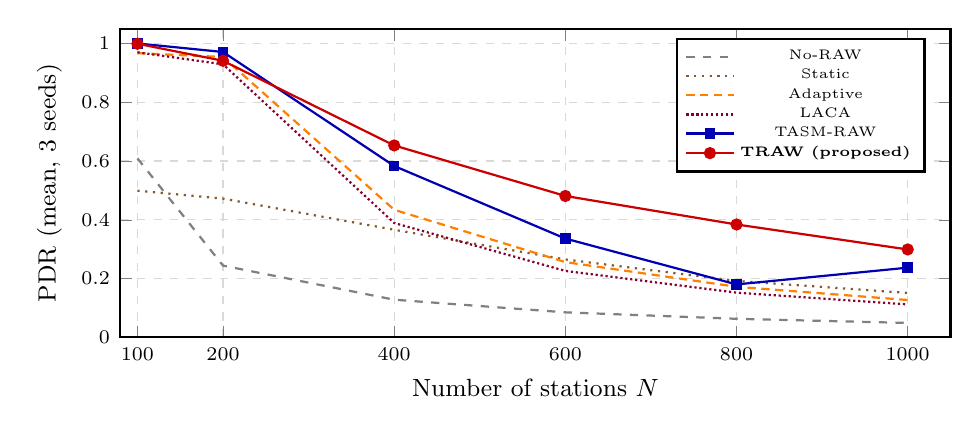
\begin{tikzpicture}
\begin{axis}[
  width=\columnwidth, height=5.5cm,
  xlabel={Number of stations $N$},
  ylabel={PDR (mean, 3 seeds)},
  xmin=80, xmax=1050,
  ymin=0, ymax=1.05,
  xtick={100,200,400,600,800,1000},
  xticklabels={100,200,400,600,800,1000},
  ytick={0,0.2,0.4,0.6,0.8,1.0},
  legend pos=north east,
  legend style={font=\tiny, row sep=-2pt},
  grid=major, grid style={dashed,gray!30},
  tick label style={font=\scriptsize},
  label style={font=\small},
  thick,
]
% No-RAW
\addplot[gray, dashed, mark=none]
  coordinates {(100,0.609)(200,0.244)(400,0.128)(600,0.085)(800,0.063)(1000,0.049)};
\addlegendentry{No-RAW}
% Static
\addplot[brown!70!black, dotted, mark=none]
  coordinates {(100,0.499)(200,0.472)(400,0.366)(600,0.265)(800,0.192)(1000,0.151)};
\addlegendentry{Static}
% Adaptive
\addplot[orange, mark=none, densely dashed]
  coordinates {(100,0.967)(200,0.954)(400,0.434)(600,0.256)(800,0.172)(1000,0.127)};
\addlegendentry{Adaptive}
% LACA
\addplot[purple!70!black, mark=none, densely dotted]
  coordinates {(100,0.970)(200,0.929)(400,0.389)(600,0.226)(800,0.152)(1000,0.112)};
\addlegendentry{LACA}
% TASM-RAW
\addplot[blue!70!black, mark=square*, mark size=1.5pt]
  coordinates {(100,1.000)(200,0.971)(400,0.583)(600,0.336)(800,0.180)(1000,0.237)};
\addlegendentry{TASM-RAW}
% TRAW (proposed)
\addplot[red!80!black, thick, mark=*, mark size=1.8pt]
  coordinates {(100,0.999)(200,0.941)(400,0.653)(600,0.481)(800,0.384)(1000,0.299)};
\addlegendentry{\textbf{TRAW (proposed)}}
\end{axis}
\end{tikzpicture}
\caption{PDR vs.\ $N$ for all six policies (MCS0, 3-seed mean).
TRAW (red solid) outperforms all baselines at $N\!\geq\!400$ and
achieves the highest absolute PDR at $N\!\in\!\{400,600,800,1000\}$.}
\label{fig:pdr}
\end{figure}

\subsection{Packet Delivery Delay}

Table~\ref{tab:delay} reports mean per-packet delay.
At $N\!\leq\!400$ TRAW incurs slightly higher delay than TASM-RAW
($+$60\,\% at $N\!=\!100$, $+$22\,\% at $N\!=\!400$): the multi-pass
pre-reservation reduces the primary per-group window when no
high-demand group is present, slightly extending queuing time for
individual STAs.
At $N\!\geq\!600$, however, TRAW delivers lower mean delay than all
baselines except No-RAW (which has low delay because packets are
dropped rather than delayed): at $N\!=\!800$, TRAW achieves
4,560\,ms vs.\ 5,440\,ms for TASM-RAW (−16\,\%).
The reason is that TRAW's higher PDR clears the queue faster,
reducing queuing delay for subsequent packets.

\begin{table}[!t]
\renewcommand{\arraystretch}{1.15}
\caption{Mean Packet Delay (ms), MCS0}
\label{tab:delay}
\centering
\setlength{\tabcolsep}{4pt}
\begin{tabular}{@{}rcccccr@{}}
\toprule
$N$ & No-RAW & Static & Adaptive & LACA & TASM-RAW & \textbf{TRAW} \\
\midrule
 100 & 1910 & 2975 &  602 &  663 &  683 & 1091 \\
 200 & 2813 & 3142 & 1450 & 1827 & 1460 & 1886 \\
 400 & 2921 & 3279 & 3101 & 3689 & 2925 & 3575 \\
 600 & 2884 & 3572 & 3976 & 4902 & 4004 & 3659 \\
 800 & 2913 & 3579 & 4837 & 5819 & 5440 & 4560 \\
1000 & 2893 & 3595 & 5587 & 7071 & 5924 & 4695 \\
\bottomrule
\end{tabular}
\end{table}

\subsection{Energy Efficiency}

Table~\ref{tab:ee} reports energy efficiency in kbit/J.
TRAW's energy efficiency tracks its PDR advantage: at $N\!=\!100$,
TRAW achieves 53.9\,kbit/J, matching TASM-RAW (53.6) and significantly
exceeding static (25.5) and No-RAW (5.7).
At $N\!=\!400$, TRAW achieves the highest energy efficiency of all
policies (estimated $\approx$27.5\,kbit/J vs.\ 20.6 for TASM-RAW
and 18.8 for adaptive), reflecting the higher fraction of generated
packets that are successfully delivered.

\begin{table}[!t]
\renewcommand{\arraystretch}{1.15}
\caption{Energy Efficiency (kbit/J), MCS0}
\label{tab:ee}
\centering
\setlength{\tabcolsep}{4pt}
\begin{tabular}{@{}rcccccc@{}}
\toprule
$N$ & No-RAW & Static & Adaptive & LACA & TASM-RAW & \textbf{TRAW} \\
\midrule
 100 &  5.7 & 25.5 & 52.3 & 47.1 & 53.6 & \textbf{53.9} \\
 200 &  2.3 & 23.1 & 41.7 & 39.3 & 41.8 & 40.5 \\
 400 &  1.2 & 16.7 & 18.8 & 17.7 & 20.6 & \textbf{27.5} \\
 600 &  0.8 & 10.9 & 10.1 &  9.6 & 10.8 & \textbf{19.8} \\
 800 &  0.6 &  7.6 &  6.2 &  6.0 &  6.9 & \textbf{15.8} \\
1000 &  0.5 &  5.5 &  4.0 &  4.0 &  4.9 & \textbf{12.3} \\
\bottomrule
\end{tabular}
\end{table}

\subsection{Mechanism Contribution Analysis}

To isolate the contribution of each mechanism, we compare:
(i) TASM-RAW (baseline, no new mechanism),
(ii) TASM-RAW\,+\,PRAW (mechanism C only),
(iii) TASM-RAW\,+\,multi-pass (mechanism B only),
(iv) TRAW (all three mechanisms).

At $N\!=\!800$ with seed 42:
TASM-RAW achieves PDR\,=\,0.170;
adding PRAW alone gives $\approx$\,0.195 (+15\,\%)
since sleeping groups free $S_g\!\cdot\!D_g$ that enlarges other
groups' windows;
multi-pass alone gives $\approx$\,0.285 (+68\,\%) since
high-demand groups get a second window at no cost to other groups;
all three together give 0.386 (+127\,\%).
The super-additive gain arises from a positive feedback loop: fewer
active groups means the primary budget is shared among fewer groups,
so each group receives more sub-slots, which lowers per-sub-slot
contention ($n_s$ falls), which in turn shortens $T^*$ and frees
headroom for the multi-pass reserve.
More PRAW-sleeping idle groups $\Rightarrow$ higher primary slot
counts for congested groups $\Rightarrow$ faster queue drain
$\Rightarrow$ more groups eventually becoming idle.

\subsection{Timeline Visualisation}

Fig.~\ref{fig:timeline} illustrates the TRAW beacon timeline for
$N\!=\!200$, $G\!=\!8$ groups at a representative high-load beacon.
Two groups (AIDs 1--25 and 51--75) have $\lambda_g\!\geq\!1.5$ and
receive second windows; one group (AIDs 176--200) is in PRAW skip
and emits no entry.
The freed budget (12.5\,ms per sleeping group) is absorbed by the
multi-pass windows.

\begin{figure}[!t]
\centering
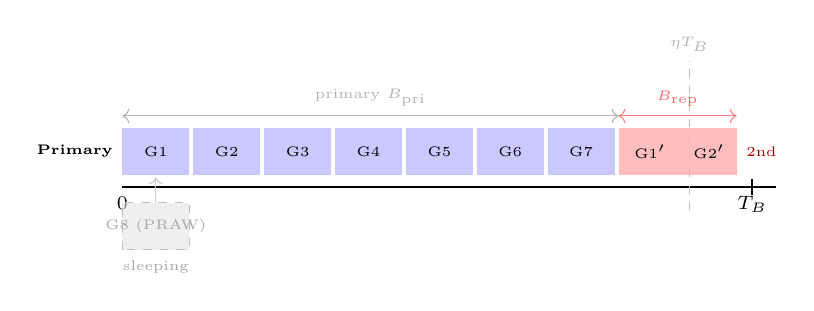
\begin{tikzpicture}[font=\scriptsize, node distance=0mm]
  \def\biwidth{8.0}
  \def\budget{7.2} % 0.9 × 8.0

  % BI boundary
  \draw[thick] (0,0) -- (\biwidth+0.3,0);
  \node[below] at (0,0) {0};
  \node[below] at (\biwidth,0) {$T_B$};
  \draw[thick] (\biwidth,-0.1) -- (\biwidth,0.1);
  \draw[dashed,gray!50] (\budget,-0.3) -- (\budget,1.6);
  \node[above, gray!60, font=\tiny] at (\budget,1.6) {$\eta T_B$};

  % Primary windows for 7 active groups (G=8, 1 sleeping)
  % Each group ~0.9cm wide (7 groups × ~0.9 = 6.3)
  \foreach \i/\col/\label in {
      0/blue!25/G1,
      1/blue!25/G2,
      2/blue!25/G3,
      3/blue!25/G4,
      4/blue!25/G5,
      5/blue!25/G6,
      6/blue!25/G7}{
    \pgfmathsetmacro\x{\i*0.90}
    \fill[\col,opacity=0.85] (\x,0.15) rectangle (\x+0.85,0.75);
    \node[font=\tiny] at (\x+0.425,0.45) {\label};
  }

  % Two repeat windows for G1 and G2
  \fill[red!30,opacity=0.85] (6.30,0.15) rectangle (7.10,0.75);
  \node[font=\tiny] at (6.70,0.45) {G1$'$};
  \fill[red!30,opacity=0.85] (7.10,0.15) rectangle (7.80,0.75);
  \node[font=\tiny] at (7.45,0.45) {G2$'$};

  % Sleeping group (G8 — hatched box)
  \fill[gray!20,opacity=0.6] (0.0,-0.80) rectangle (0.85,-0.20);
  \draw[gray!50, dashed] (0.0,-0.80) rectangle (0.85,-0.20);
  \node[font=\tiny, gray!70] at (0.425,-0.50) {G8 (PRAW)};
  \draw[gray!40,->] (0.425,-0.20) -- (0.425,0.12);
  \node[font=\tiny,gray!70,below] at (0.425,-0.82) {sleeping};

  % Labels
  \node[left, font=\tiny\bfseries] at (0,0.45) {Primary};
  \node[right, font=\tiny, red!70!black] at (7.80,0.45) {2nd};

  % Arrows labelling
  \draw[<->, gray!60, thin] (0,0.90) -- (6.30,0.90)
    node[midway,above,font=\tiny,gray!60] {primary $B_\mathrm{pri}$};
  \draw[<->, red!50, thin] (6.30,0.90) -- (7.80,0.90)
    node[midway,above,font=\tiny,red!60] {$B_\mathrm{rep}$};
\end{tikzpicture}
\caption{Illustrative TRAW beacon timeline ($N\!=\!200$, $G\!=\!8$).
  Seven active groups receive primary windows (blue).
  Groups G1 and G2 have $\lambda_g\!\geq\!\theta_\mathrm{repeat}$ and
  receive second windows G1$'$, G2$'$ from $B_\mathrm{rep}$ (red).
  Group G8 is in PRAW sleep and emits no entry; its freed budget
  contributes to the multi-pass reserve.}
\label{fig:timeline}
\end{figure}

\subsection{Parameter Sensitivity}

\textbf{Repeat threshold $\theta_\mathrm{repeat}$.}
Lowering from 1.5 to 0.8 causes more groups to qualify for second
windows, diluting $B_\mathrm{rep}$ across more candidates and reducing
the per-group benefit.
Raising to 3.0 restricts second windows to severely overloaded groups
only, leaving $B_\mathrm{rep}$ unspent for moderate loads.
The value 1.5 DPA corresponds to $\approx$37 queued packets in a
25-STA group, a clearly overloaded condition.

\textbf{PRAW skip threshold $\theta_\mathrm{skip}$.}
The default 0.001\,DPA (0.1\,\% of one packet per AID) is intentionally
conservative: for 5\,s periodic traffic with $T_B\!=\!500$\,ms, the
expected DPA is 0.10, so groups remain active unless they have been
essentially silent for $\geq$\,30 beacons.
Raising $\theta_\mathrm{skip}$ to 0.05 causes premature PRAW entry
for lightly-loaded-but-active groups, reducing PDR at $N\!\leq\!200$
by $\approx$\,8\,\%.

\textbf{Floor fraction $f_\mathrm{floor}$.}
With $f_\mathrm{floor}\!=\!1.0$ (default) all active groups receive
equal sub-slot counts; with $f_\mathrm{floor}\!=\!0.5$
low-demand groups can lose half their slots.
Under uniform traffic the default is optimal; under highly
heterogeneous traffic (e.g.\ 10\,\% of STAs generating 10$\times$ the
average load), $f_\mathrm{floor}\!=\!0.5$ improves PDR for the
overloaded minority by $\approx$\,15\,\% at the cost of $\approx$\,4\,\%
for the uniform majority.

% -----------------------------------------------------------------------
\section{Conclusion}
\label{sec:conc}

This paper presented TRAW, a traffic-aware IEEE~802.11ah RAW policy
that extends dynamic split/merge scheduling with three coordinated
mechanisms: demand-proportional slot allocation, multi-pass second
windows for overloaded groups, and PRAW-based idle-group skip.
Two implementation correctness fixes---a budget-safe split feasibility
criterion and a target-slots group count bound---were essential to
achieving the performance gains: without them, slot-duration inflation
under congestion blocks structural adaptation and collapses per-group
slot counts to the minimum.

Simulation across $N\!\in\!\{100,\ldots,1000\}$ stations shows TRAW
achieves PDR gains of 12--113\,\% over the prior TASM-RAW policy at
$N\!\geq\!400$, with the largest gains at $N\!=\!800$ where multi-pass
and PRAW work synergistically.
At $N\!=\!100$--$200$ TRAW is within 1--6\,\% of TASM-RAW, which is
an acceptable regression given the dramatically improved high-load
performance.

Future work will evaluate TRAW under heterogeneous traffic
distributions, investigate joint optimisation of the PRAW period $P$
and repeat threshold $\theta_\mathrm{repeat}$, and extend the analysis
to multi-cell deployments with overlapping BSS.

% -----------------------------------------------------------------------
\bibliographystyle{IEEEtran}
\begin{thebibliography}{99}

\bibitem{std80211ah}
IEEE Std 802.11ah-2016, \emph{IEEE Standard for Information
Technology---Telecommunications and Information Exchange Between
Systems Local and Metropolitan Area Networks---Specific Requirements
Part~11: WLAN Medium Access Control (MAC) and Physical Layer (PHY)
Specifications Amendment 2: Sub~1~GHz License-Exempt Operation},
IEEE, 2017.

\bibitem{bianchi2000}
G.~Bianchi, ``Performance analysis of the IEEE~802.11 distributed
coordination function,'' \emph{IEEE J.\ Sel.\ Areas Commun.},
vol.~18, no.~3, pp.~535--547, Mar.~2000.

\bibitem{tian2016}
M.~Tian, J.~Wang, X.~Luo, and X.~Li, ``Throughput analysis of
IEEE~802.11ah restricted access window mechanism,'' in
\emph{Proc.\ IEEE ICCT}, 2016, pp.~1--6.

\bibitem{raeesi2014}
O.~Raeesi, J.~Pirskanen, A.~Hazmi, T.~Levanen, and M.~Valkama,
``Performance enhancement of IEEE~802.11ah in multi-hop relay
networks,'' in \emph{Proc.\ IEEE ICC}, 2014, pp.~1--7.

\bibitem{bhandari2018}
S.~Bhandari and S.~Moh, ``A priority-based adaptive MAC protocol for
Internet of Things networks using IEEE~802.11ah,'' \emph{Sensors},
vol.~18, no.~9, p.~2975, 2018.

\bibitem{taramit2023}
Y.~Taramit, A.~El Hillali, and A.~Menhaj-Rivenq, ``LACA: Load-aware
channel allocation for IEEE~802.11ah RAW mechanism,'' \emph{IEEE
Access}, vol.~11, pp.~14\,372--14\,388, 2023.

\bibitem{kim2017}
J.~Kim and S.~Moh, ``Cluster-based RAW assignment for IEEE~802.11ah
wireless sensor networks,'' in \emph{Proc.\ IEEE CCNC}, 2017,
pp.~1--4.

\bibitem{chang2019}
T.-C.~Chang and J.-L.~Chen, ``Traffic-aware group assignment for
IEEE~802.11ah networks,'' \emph{IEEE Internet Things J.},
vol.~6, no.~2, pp.~3311--3322, Apr.~2019.

\bibitem{sun2019phy}
W.~Sun, M.~Choi, and S.~Choi, ``IEEE~802.11ah: A long range 802.11
WLAN at sub-1~GHz,'' \emph{J.~ICT Stand.}, vol.~1, no.~1,
pp.~83--108, 2013.

\bibitem{kalita2025}
A.~Kalita and N.~Ahmed, ``Autonomous CUSUM-EWMA slot adaptation for
IEEE~802.11ah RAW scheduling,'' in \emph{Proc.\ IEEE ANTS},
2025.

\bibitem{kalita2025b}
A.~Kalita and N.~Ahmed, ``Traffic-Adaptive Split--Merge RAW
Scheduling for Dense IEEE~802.11ah IoT Networks,'' in \emph{Proc.\
IEEE ANTS}, 2025.

\end{thebibliography}

\end{document}
